\section{Formal verification processes applicable to a SCADE~model}

A second possibilities is to apply a formal verficiation process to  the Scade model, for this we propose an a posteriori verification based on model-checking.



\subsection{Principles of \smartsolver{}}

Systerel Smart Solver (\smartsolver{}) is a  \SAT{}-based
model checker for safety properties analysis. 

The High Level Language (\HLL{}), the input language of \smartsolver{}, is a stream oriented declarative data-flow language which can be used to  model:

\begin{itemize}
\item the system behavior
\item the environment
\item the formal expression of the properties.
\end{itemize}

\smartsolver{} proceeds to  the analyses of properties on the traces of the \HLL{} models following one of these two strategies:
\begin{itemize}
\item Induction to prove a property (see \cite{Sheeran:2000});
\item Bounded model checking (BMC) to falsify a property or generate test cases (see \cite{Biere:1999,Amla:2005}).
\end{itemize}

Thus \smartsolver{} can be applied on different ways to  verify and validate a critical industrial  system.


\subsection{Application of \smartsolver{}: Static analysis}
\label{sec:static-analysis}

\smartsolver{} adds some proof obligations to assess that the \HLL{}
model is correctly defined:
\begin{itemize}
\item Indexes of arrays belong to their ranges
\item Latch definition range check
\item No division by 0
\item No overflow and no underflow on arithmetic expressions
\item Output and constraint initialization check
\end{itemize}

Besides, the translators from a language to \HLL{} can also generate proof obligations to be analyzed by \smartsolver{},
to check that the code does not have undefined behavior with respect to the source language.

For example the C-translator adds some proof obligations to ensure conformance with the C99 standard.

\subsection{Application of \smartsolver{}: Verification of Safety Properties}
\label{sec:verif-safety-prop}

Safety Properties are of the form $always~\phi$ meaning that the Boolean
predicate $\phi$ holds Globally, \ie{}, in every state reachable from the
initial state. \smartsolver{} can be used to verify safety properties as shown
in the process in Fig.~\ref{fig:s3-safety-prop}.


\begin{figure}[h]
  \centering
  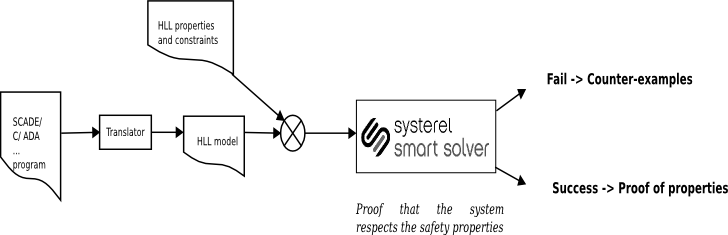
\includegraphics[width=1\textwidth]{figures/s3proof}
  \caption{Safety Property Verification}
  \label{fig:s3-safety-prop}
\end{figure}


First the source program in either \textsc{C}, \SCADE{}, Ada,... is translated
into \HLL{} format via a translator; this \HLL{} system model is then
combined with safety properties expressed in \HLL{} to form a verification
model. 
Environment hypotheses and constraints can be added if a property does not hold 
based  only on the formal model of the software and requires additional
hypotheses about the overall system and/or its environment.

Finally the properties are verified using \smartsolver{}.

A good approach is to first use the BMC strategy with a rather large depth
(depending on the system).
After, if there is no counter-example, the induction strategy can be launched.


\subsection{Application of \smartsolver{}: Equivalence Verification of Different Models}
\label{sec:equiv-verif-diff}

There are different areas where the formal verification of equivalence is
required. One such example is the verification of equivalence of two different
tool chains for the same task in an approach based on diversification. Such an
approach is often used in the development of safety critical systems, to
decrease the probability of errors. In general,  two different
versions of a software are developed independently, using different programming languages, different
approaches and also separate teams.

The equivalence of the two resulting system models is then verified using
\smartsolver{}. 

To prove equivalence between two \HLL{} models, we make the hypothesis
that the inputs of the two \HLL{} models are equal and we want to prove
that the outputs are equal (see Fig.~\ref{fig:s3-equiv-check}).


\begin{figure}[h]
  \centering
  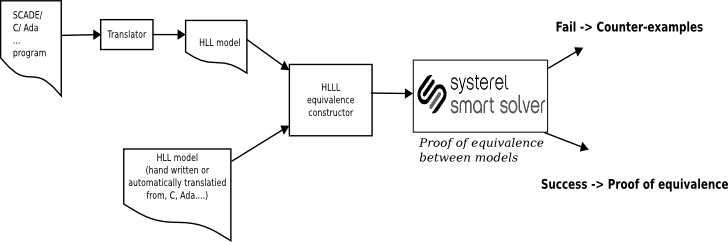
\includegraphics[width=1\textwidth]{figures/s3equiv}
  \caption{Equivalence Check}
  \label{fig:s3-equiv-check}
\end{figure}


The equivalence could also be used to prove that a code is equivalent to
a specification: the code is translated into \HLL{} and the
specification is written in \HLL{}.

It is also used in the certification flow (see section~\ref{cs3}).


\subsection{Application of \smartsolver{}: Test Case Generation}
\label{sec:test-case}

\smartsolver{} can also be used for test case generation:
\begin{itemize}
\item In the case of functional black-box testing, the main difficulty in writing of test scenario is to  define the values of the outputs to observe as a function of the input values, as the analysis of the functionality can be complex.
\item In the case of white-box verification, the difficulty is to define the right input values to cover a function, a branch or a condition.
\end{itemize} 



As an alternative, for black box-testing, \smartsolver{} shall allow to determine easily test oracle.
For white-box testing, we can easily write a test objective in \HLL{} that
states exactly the objective of the test (e.g. the desired output values). Applying a BMC strategy, we obtain all the desired scenario with the expected values of the inputs.


\subsection{Certifiable Systerel Smart Solver}
\label{cs3}

In order to conform to industrial standards  requirements for critical systems~\cite{standard_railway_2011,standard_aerospace_2011}, we propose a certifiable formal verification solution with  \smartsolver{} (see Fig.\ref{fig:s3-certif-check}).


\begin{figure}[h]
  \centering
  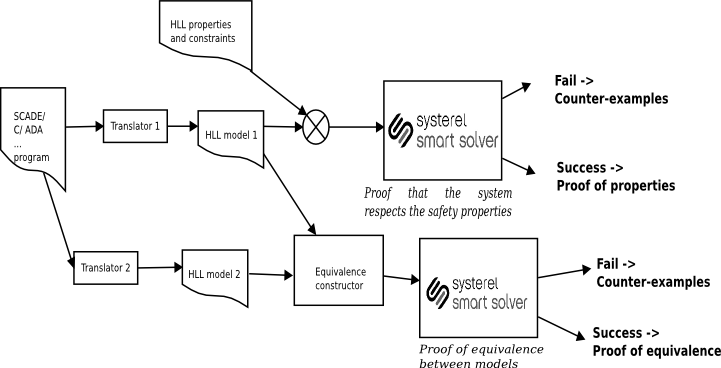
\includegraphics[width=1\textwidth]{figures/s3certif}
  \caption{Certifiable solution}
  \label{fig:s3-certif-check}
\end{figure}

When building certifiable formal verification
solutions, the certifiable Systerel Smart Solver (c\smartsolver{}) approach relies on three different techniques:
\begin{description}
\item [Diversification of the translation chain:] the translation of a model to \HLL{} is
  done twice\footnote{When applicable, these diversified translations
    are performed from differentiated sources.}, with two
  translators being developed by two independent teams in two  independent programming language (for instance one in C the other in Ocaml). 
\item [Equivalence-check of the translated models:] the  outputs of the two diversified
  translation chains are compared using equivalence
  checking. \smartsolver{} is used together with an equivalence-constructor to check if
  the two translated models are {\em sequentially equivalent}, \ie, if
  given the same scenario on their inputs, they would produce the same
  outputs.
\item [Record of results in a verifiable proof-log:] when a proof is validated or an equivalence between model established, the result of the \smartsolver{} is not a simple  ``OK'' answer, but a {\em proof-log} file that
  contains an encoding of the proof of this claim in a sound and
  complete proof-system. An independent checker is run
  \textit{a-posteriori} to check the correctness of this proof.
\end{description}





\subsection{Application on Modes and Levels function}

The approach has been applied on Modes and Levels function modelled in Scade (\footnote{\url{https://github.com/openETCS/modeling/tree/master/model/Scade/System/ObuFunctions/ManageLevelsAndModes}})

\begin{tabular}{|l|l|l|l|l}
\hline
\textbf{Name} & \textbf{Type} & \textbf{Model} & \textbf{SRS coverage} & \textbf{section} \\ \hline
isolate & simple proof & Modes  & 4.6.2 C1 &\\
no\_power & simple proof & Modes  & 4.6.2 C4 &\\
level case & use case & Level  & 5.10 &\\
shunting initiated by driver & validation & Modes  & 5.6 &\\
start of mission & validation & Modes  & 5.4 &\\
%\hline
%ManageModes & start\_of\_mission\_topnode.hll \\
\hline
\end{tabular}


\subsubsection{Application of \smartsolver{}: Static analysis}
\label{sec:static-analysis}

At first, the formal verification of the model was used to find bugs in the developed
\SCADE{} model.
\smartsolver{} adds some proof obligations to assess that the \HLL{}
model is correctly defined:
\begin{itemize}
\item Indexes of arrays belong to their ranges
\item Latch definition range check
\item No division by 0
\item No overflow and no underflow on arithmetic expressions
\item Output and constraint initialization check
\end{itemize}

Besides, the translators from a language to \HLL{} can also generate proof obligations to be analyzed by \smartsolver{},
to check that the code does not have undefined behavior with respect to the source language.

For example the C-translator adds some proof obligations to ensure conformance with the C99 standard.


\paragraph{Results}
The three models have been verified on their topnode:

\begin{tabular}{|l|l|l|}
\hline
\textbf{\SCADE{} model} & \textbf{Top Node} & \textbf{Results}  \\ \hline
Modes & ManageModes &  PO 1-5: valid \\
Levels & ManageLevels &  PO 1-5: valid \\
ModesAndLevels & ManageLevelAndMode & PO 1-5: valid \\
\hline
\end{tabular}

\subsubsection{Conditions to Isolate mode}
\label{sec:isolate}

\paragraph{Files used for the proof} The proof is defined in the file \url{https://github.com/openETCS/validation/blob/master/VnVUserStories/VnVUserStorySysterel/05-Work/S3/Small_Proof/isolate.hll} and it is verified on the top node \emph{ManageModes} of the \SCADE{} model \emph{Modes}.


\paragraph{What is proved ?}
The Condition 1 of SRS § 4.6 "The driver isolates the ERTMS/ETCS on-board equipment" is proved, ie; as soon as the input of \SCADE{} model \texttt{Data\_From\_DMI.'ETCS\_Isolated'} becomes true, the output \texttt{currentMode} becomes 'isolated' (\texttt{Level\_And\_Mode\_Types\_Pkg::IS}) and internal condition  is activated.


\paragraph{Constraints used}

None.

\paragraph{Results}

The property is proved.


\subsubsection{Procedure Shunting initiated by Driver}

\paragraph{Files used for the proof} The proof is defined in the file \url{https://github.com/openETCS/validation/blob/master/VnVUserStories/VnVUserStorySysterel/05-Work/S3/Proof_SoM/shunting_initiated_by_driver.hll} and it is verified on the node \emph{Procedure\_SH\_Initiated\_By\_Driver} of the \SCADE{} model \emph{Modes Management}. The same proof is also defined in the file \url{https://github.com/openETCS/validation/blob/master/VnVUserStories/VnVUserStorySysterel/05-Work/S3/Proof_SoM/shunting_initiated_by_driver_topnode.hll} to be verified on the top node \emph{ManageModes} of the \SCADE{} model \emph{Modes Management}.

\paragraph{What is proved ?}
We want to prove that the procedure SH\_Initiated\_By\_Driver is a
correct implementation of the section 5.6 Shunting Initiated By Driver of SRS-26.

To prove this, a specification of the flowchart is proposed in the
property file. However, the flowchart is not entirely specified:
elements \texttt{D030}, \texttt{A030}, \texttt{A095}, \texttt{S100} and
\texttt{A115} of the flow chart in SRS-26 are out of the scope of the mode management function.

\paragraph{Constraints used}
One hypothesis is used in this model to avoid a counter-example: when we are in \texttt{A100} the request of ``End of
Mission'' procedure correspond to the value of the input
\texttt{On-going Mission} as it is specified in the \SCADE{} model.

This hypothesis is justified by the fact that, according to
\texttt{A050}, \texttt{D040} and \texttt{A100}, if the input
\texttt{On-going Mission} is \texttt{True} then the ``End of Mission''
request is \texttt{True}, so equal to \texttt{On-going Mission}. Also,
as transition to SH mode is enable (\texttt{A050}) when ``End of
Mission'' request is made, the system should go to SH mode (or another
mode except SB mode). 

\paragraph{Results}
Considering the constraint and our model, the \SCADE{} model of
SH\_Initiated\_By\_Driver corresponds to the specification. Proof of this property allow to detect an error in \SCADE{} model: operator \emph{AND} was used instead operator \emph{OR}.
Besides the specification in \SCADE{}  of the computation of the output \emph{End\_Of\_Mission} was corrected.

\subsubsection{Procedure Start of Mission}

\paragraph{Files used for the proof}
The proof is defined in the file \url{https://github.com/openETCS/validation/blob/master/VnVUserStories/VnVUserStorySysterel/05-Work/S3/Proof_SoM/startofmission_topnode_proof.hll} and it is verified on the node \emph{Procedure\_StartOfMission} of the \SCADE{} model \emph{Modes}.


\paragraph{What is proved ?}
We want to prove that the procedure Procedure\_StartOfMission is a
correct implementation of the section 5.6 Procedure Start of mission of SRS-26.

Only the down part of the flowchart, from S10 and from S20, relative to the modes management, is specified in the \SCADE{} model.





\paragraph{Constraints used}
\begin{enumerate}
\item Level should not change : Level can be change at the beginning of Start of Mission procedure, but when we go in the step of mode selection, the level should not change.

\item Train Data should not change : Train Data are validated at the beginning of Start of Mission procedure, they shall be valid to start mode selection and we consider then that  their validity should not change.

\item The train shall stay at standstill during all the procedure. Indeed in Stand-By mode, standstill shall be ensure by supervision function (see SRS-26 §4.4.7.1.5).

\item The ``On Going Mission'' variable, input of SH Initiated by Driver, is
forced to False. This is justified by SRS 5, section ``5.4.6 Entry to
Mode Considered as a Mission''.
\end{enumerate}



\paragraph{Results}
Considering constraints and our \HLL{} model, the \SCADE{} model of Procedure
Start of Mission corresponds to the specification.
Some errors have been detected in the \SCADE{} model: links between nodes were wrong.


\subsection{Conclusion}




Benefits of formal  methods in an a posteriori verification process of critical systems has been recognized by our industrial customers:

\begin{itemize}
\item Contrarily to a human generated test-based verification solution, a formal safety verification is
intrinsically complete. It is equivalent to search for every possible falsification.
\item It clearly identifies the complete list of assumptions upon which the safety relies.
\item A certified solution allows for a reduction of the testing and review efforts (only the generic safety
specification has to be reviewed).
\item The use of formal verification in the qualification of critical software sends a strong
and positive message to the market, and is sometime even a requirement for some customers.
\end{itemize}


